\subsubsection{Modelo de grafos}
    \label{sec:RTM}
    
    Otros estudios han tratado de modelar el trazado ferroviario utilizando teoría de grafos en el pasado [REF]. Pero todos ellos definían a las vías como las aristas del grafo y los cambios de vías como los nodos, lo cual dificultaba enormemente la inclusión de otros elementos ferroviarios como las plataformas, los pasos a nivel o los semáforos. RailTopoModel se apega mas a la teoría clásica de grafos y define como nodos a la unidad mínima de recursos físicos, llamándolos netElements y a la conexión física entre ellos como aristas, llamándolos netRelations.

    Un netElement debe contener un tramo de vía en su totalidad o varios tramos, pero un tramo de vía no puede tener varios netElements asociados. Opcionalmente, un netElement puede tener, además cualquier otro elemento ferroviario asociado como plataformas, semáforos o balizas. Para entender mejor como se materializa este concepto se tiene la Figura \ref{fig:grafos_1} que ejemplifica el modelado en grafos de una maquina de cambios.

    \begin{figure}[!h]
        \centering
        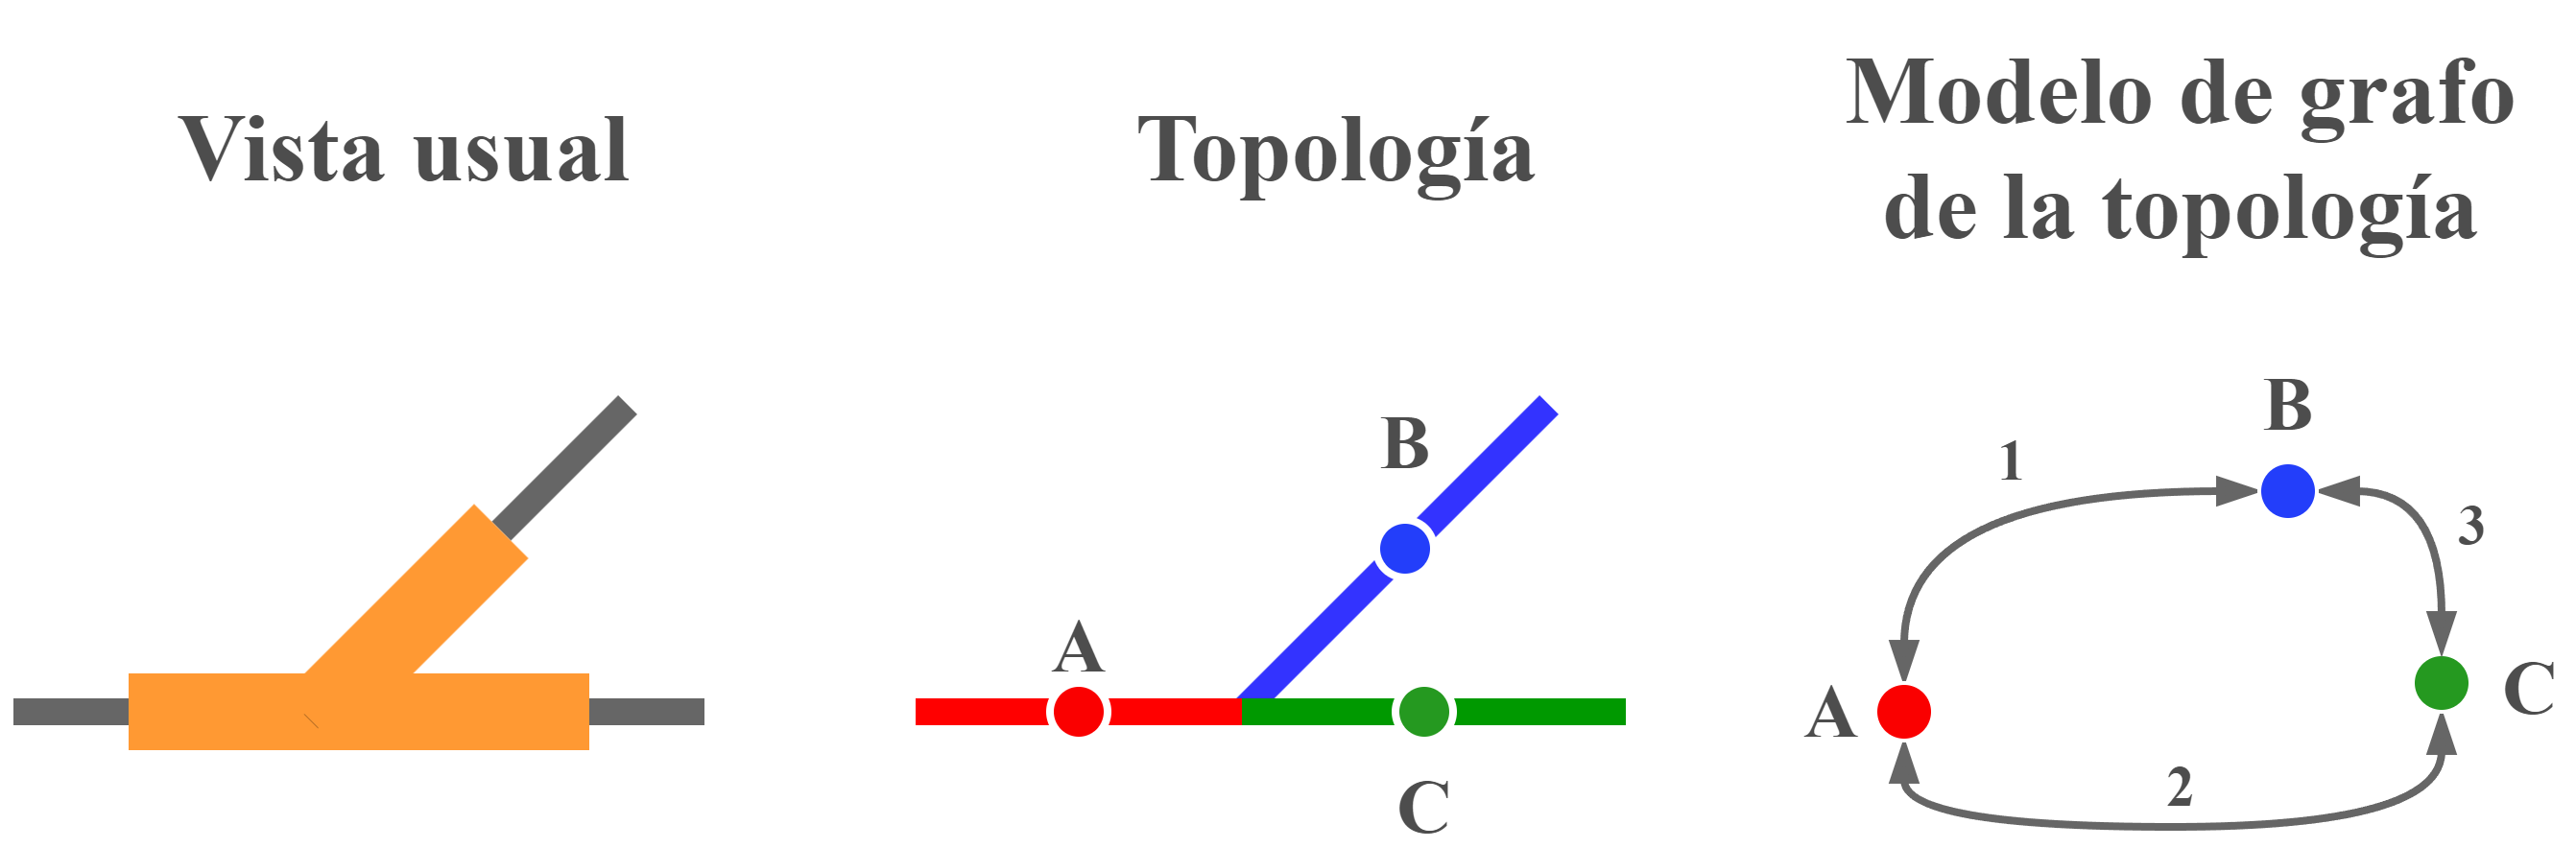
\includegraphics[width=1\textwidth]{Figuras/grafos}
        \centering\caption{Modedelado en grafos de una máquina de cambios simple.}
        \label{fig:grafos_1}
    \end{figure}

    En la Figura \ref{fig:grafos_1} se tiene una máquina de cambios simple que conecta una vía de circulación (horizontal) con una vía de maniobras (oblicua). El netElement asociado a la vía principal antes de la bifurcación lo llamaremos A. Este netElement es también al que se asocia al objeto de la máquina de cambios. El netElement asociado a la vía de maniobras lo denominamos B y al asociado a la vía de continuación de la cirlación lo denominamos C.

    En la representación del modelo de grafos, el netRelation 1 relaciona el netElement A y B de forma biyectiva. Es decir, A esta relacionado con B y B está relacionado con A. De la misma forma se asignan los netRelations 2 y 3. Sin embargo, no hay que confundir que dos vías estén conectadas con que un tren puede circular por ellas. Una formación podría circular por el tramo A-C, A-B, B-A y C-A, pero no podrá circular desde B hacia C sin pasar por A o viceversa. Es físicamente imposible que un tren realice ese movimiento de una sola maniobra. Para circular desde B hacia C primero deberá finalizar el tramo B-A, modificar la posición de la máquina de cambios y recorrer el tramo A-C. A la propiedad asignada a los netRelation que son físicamente transitables se la denomina navegabilidad y es una característica esencial de las redes de grafos que modelan redes ferroviarias. En este ejemplo, solo los netRelation 1 y 2 poseen navegabilidad.